\ifx\headerIncludedJR\undefined
  \documentclass[11pt,a4paper]{article}
  \setlength{\textwidth}{5.50in}
  \usepackage[utf8]{inputenc}
\usepackage[T1]{fontenc}
\usepackage{amsmath}
\usepackage{amsthm}
\usepackage{amssymb}
%\usepackage{rotating}
%\usepackage{amslatex}
\usepackage{siunitx}
\usepackage{multicol}%for multicol
\usepackage{blkarray}%blockarray and block
\usepackage{comment}
\usepackage{fnbreak}%get a warning if a footnote is split
\usepackage[section]{placeins}
\usepackage{listings}
\lstset{breaklines=true,basicstyle=\ttfamily,language=Python}
\usepackage{arrayjobx}
\usepackage{array}%for \newcolumntype
%\usepackage[shortlabels]{enumitem}
\usepackage{mathtools}
\usepackage{afterpage}
\usepackage{setspace}% for \setstretch
\usepackage{algorithm}
\usepackage{algpseudocode}%for algorithmic
\usepackage{thmtools}%so that autoref works with Lemmas
\usepackage{tikz}
\usepackage{pgfplots}
\pgfplotsset{compat=1.15}
\usepackage{shuffle}
\usepackage{textcomp}%for \textrecipe
\usepackage{fontawesome}%for \faTable
\usetikzlibrary{calc,shapes,arrows.meta,decorations.markings,arrows}
\usetikzlibrary{graphs,positioning,svg.path,backgrounds}
\newcommand{\tikzmark}[1]{\tikz[overlay,remember picture] \node (#1) {};}
%\usepackage{CJKutf8}%for CJKChar

%\usepackage[backend=biber,backref=true]{biblatex}
\usepackage[backend=biber,style=alphabetic,backref=true,maxbibnames=10]{biblatex}
\addbibresource{sigs.bib}
\usepackage{url}

\usepackage{imakeidx}
%not a list of definitions, just symbols and abbreviations
%What is an abbreviation? Is QR? 
\makeindex[intoc,title=Symbols and abbreviations index]
\def\jind#1{\index{#1}}
\def\jindmath#1#2{\index{#2@$#1$}}
\def\jindv#1{\index{#1v@\texttt{#1}}}
%Some places I've given up and used \index in the text 
\definecolor{bluee}{rgb}{0.4, 0.4, 1.0}
%https://tex.stackexchange.com/questions/134191/line-breaks-of-long-urls-in-biblatex-bibliography
\setcounter{biburlucpenalty}{8000}
\setcounter{biburllcpenalty}{8000}

\usepackage{hyperref}

%so that autoref works with algorithms
\newcommand{\algorithmautorefname}{Algorithm}

%might help url breaking in bibliography
%\Urlmuskip=0mu plus 1mu minus 1mu
%also all the emergencystretch/looseness/fussy/sloppy
%to play with
%https://tex.stackexchange.com/questions/18505/how-to-use-sloppy-for-just-some-references

\def\ii{{\texttt{iisignature}}}
\def\pypi{{\texttt{PyPI}}}
\def\numpy{{\texttt{numpy}}}
\def\scipy{{\texttt{scipy}}}
\def\i#1{\index{#1@\texttt{#1}}}
\def \hilite#1{\underline{\color{blue}\textbf{#1}}}
%\def \alph#1{{\color{blue}\mathbf{#1}}}
\def \lex{<_L}
\def\kron{\underline{\otimes}}

\graphicspath{{C:/Users/Jeremy/Dropbox/phd/graphs/}{/home/jeremyr/Dropbox/phd/graphs/}{/Users/reizenstein/DropboxPersonalSymlink/phd/graphs/}}

%\RequirePackage{relsize}
%\DeclareRobustCommand\CXX{C\kern-.05em \raisebox{.3ex}{\scalebox{0.9}{\textbf{+\kern-.10em+}}}}
\DeclareRobustCommand\CXX{C\kern-.05em {\scalebox{0.9}{\textbf{+\kern-.10em+}}}}
%\DeclareRobustCommand\{\texorpdfstring{\CXX}{C++}}
\DeclareRobustCommand\CC{C\texttt{++}}
\def\bftab{\fontseries{b}\selectfont}
\newtheorem{theorem}{Theorem}
%\newtheorem*{theorem*}{Theorem}%bad idea, because you can't refer to it.
\newtheorem{definition}[theorem]{Definition}
%\newtheorem{outsideTheorem}[theorem]{Theorem}
\newtheorem{example}[theorem]{Example}
\newtheorem{conjecture}[theorem]{Conjecture}
\newtheorem{lemma}[theorem]{Lemma}
\newtheorem{proposition}[theorem]{Proposition}
\newtheorem{remark}[theorem]{Remark}

\newcommand{\area}{\mathsf{area}}
\newcommand{\Area}{\mathsf{Area}}
\newcommand{\emptyword}{\epsilon}
\newcommand{\ds}{d} % dimension of the signal
\newcommand{\TC}{T((\R^\ds))} % concat
\newcommand{\TS}{T(\R^\ds)} % shuffle
\newcommand{\GL}{\operatorname{GL}}
\newcommand{\SO}{\operatorname{SO}}
%\newcommand{\id}{\operatorname{id}}
\newcommand{\id}{\mathsf{id}}

\newcommand{\evaluatedAt}[1]{\,\raisebox{-.5em}{$\vert_{#1}$}}

\def\hssymbol{\mathbin{\succ}}
\def\hs#1#2{#1\hssymbol#2} %half shuffle
%\def\hs#1#2{z(#1,#2)} %half shuffle
\def\areab#1{\underline{\area}(#1)}
\def\areabb{\underline{\area}}
\newcommand{\R}{\mathbb{R}}
\newcommand{\Q}{\mathbb{Q}}
\newcommand{\C}{\mathbb{C}}
\newcommand{\N}{\mathbb{N}}
\newcommand{\spann}{\operatorname{span}}
\newcommand{\sign}{\operatorname{sign}}

\DeclareMathOperator*{\argmax}{arg\,max}
\DeclareMathOperator*{\argmin}{arg\,min}
\DeclareMathOperator{\softmax}{softmax}

%indicate that this file has been had
\def\headerIncludedJR{}
\def\endDocumentJR{}

%general hints
%https://homepages.inf.ed.ac.uk/imurray2/compnotes/latex.html

  %this cannot be in header.tex as it messes up
  %the thesis copyright page
  \def \alph#1{{\color{bluee}\mathbf{#1}}}
  \begin{document}
  \tableofcontents
  \def\endDocumentJR{\printindex \printbibliography[heading=bibintoc]\end{document}}
\fi

\section{Backpropagation and derivatives}
\label{sec:backprop}
When training neural networks, it is required to calculate the gradient of a scalar function of many variables. 
The context for this will be fleshed out in \autoref{sec:minibatchesSGD}.
This is done using the chain rule in a structured fashion, known as \emph{reverse automatic differentiation} or \emph{backpropagation}.
%Backpropagation is the process of using the chain rule to find the derivative of a
In order to be able to do signature calculations inside neural networks, we need to do backpropagation of derivatives through the calculation.
The key for this is that for each calculation which takes a number of inputs to a number of outputs, we need to be able to take the derivatives of some scalar function, say $F$, of the outputs to the derivatives of that function of the inputs.
Explicitly, if as a general component of a neural network we wish to have a function\footnote{A function may take scalar inputs or other inputs with respect to which we do not need derivatives, in which case these extra inputs can be inputs to its backpropagation operation and no special extra difficulty is caused.}
\begin{align*}
f:\R^n&\to\R^m\\
f:(x_1,\dots,x_n)&\mapsto(f_1,\dots,f_m)
\shortintertext{then we need to calculate a backpropagation operation}
\overleftarrow{f}:\Big(\frac{\partial F}{\partial f_1},\dots,\frac{\partial F}{\partial f_m}\Big)&\mapsto \Big(\frac{\partial F}{\partial x_1},\dots,\frac{\partial F}{\partial x_n}\Big)\\&\qquad=\Big(\sum_i\frac{\partial F}{\partial f_i}\frac{\partial f_i}{\partial x_1},\dots,\sum_i\frac{\partial F}{\partial f_i}\frac{\partial f_i}{\partial x_n}\Big)
\end{align*}
where all partial derivatives are evaluated at a single set of inputs to the whole function $F$, and these inputs and the corresponding $(x_1,\dots,x_n)$ and $(f_1,\dots,f_m)$ can be made inputs to $\overleftarrow{f}$.  
In this section I discuss ways I have done that efficiently for some functions in \ii.
In particular, for many functions $f$ in practice it is not necessary to calculate or store every element $\frac{\partial f_i}{\partial x_j}$ of the Jacobian. 
%We have described the core functionality of \ii, the calculation of signatures and log signatures. 
\ii\ has a simple method \verb|sigjoin| for concatenating a segment onto a signature, and \verb|sigscale| for transforming a given signature according to the path being scaled by an enlargement in each of the coordinate directions. It is these and the core \verb|sig| and \verb|logsig| functions which \ii\ provides backpropagation for. 

\subsection{General thoughts}
Having a backpropagation function along with a library function can often be more efficient than defining the whole operation in the language of an autodifferentiation facility like those in \verb|tensorflow|, \verb|torch| or \verb|theano|. There are lots of steps in signature calculations which would each have to be analysed separately, and this process would probably happen every time a program was run. Each calculation we provide together with its backprop counterpart can be thought of by the deep learning library as a sealed unit. Often we can save memory this way -- we don't have to store every single intermediate value, and at runtime we don't need to work out which intermediate values need to be stored. Our function can be provided to an autodifferentiation facility as a sealed unit.

The most common style is for a backprop function to receive the original function's inputs. We have functions which have optional positional arguments. Therefore it is most consistent to take the gradient as the first argument of backprop functions followed by the original inputs. In practice, a backprop function could additionally accept original function's output and the autodifferentiation systems would be able to provide it, 
but we don't have a need to make use of this. %check
Ideally state which is internal to the calculation should not need to be remembered.

In some cases, by thinking carefully about the backpropagation operation $\overleftarrow{f}$ we can find a more sensible way to calculate it than the obvious way. This means that our own function can be more efficient than that which an autodifferentiation system is likely to have come up with. In practice, it seems that our $\overleftarrow{f}$ pleasingly take about the same time as the corresponding forwards operation $f$, and it would be unlikely that the backpropagation operation would be much quicker in any case.

When we have a calculation structure which looks like \autoref{fig:depends} to backpropagate derivatives through, we need the value of the output of each calculation of function $f$ as we pass derivatives down the tree, in order to send the derivative to the input which is a sibling of that $f$. There are basically two ways to make this available. The standard way is that we evaluate the calculation forwards storing all the intermediate $f$ values. This may require extra memory and copying of data to store them (unless we repeatedly do parts of the calculation). This is classic reverse-mode automatic differentiation in action, and is what typical deep learning packages do by default to implement backpropagation. Some of the storage can be omitted in return for redoing parts of the calculation. In some cases, however, we might be lucky, in that both $f$ and (right multiplication by something fixed) are invertible, and so we can find the output of each $f$ down the tree starting from the output of the calculation. By doing this in tandem with the backpropagation of derivatives, we don't need any storage for each level of the calculation graph. This idea works for \verb|sig| but not for
%\verb|logsigfromsig|%CHECK
converting a signature to a log signature using the series for log,
 fundamentally because among group-like elements of tensor space, multiplication by a given element is invertible, but among Lie elements, multiplication by a given element is not.

\begin{figure}[h]
	\begin{center}
		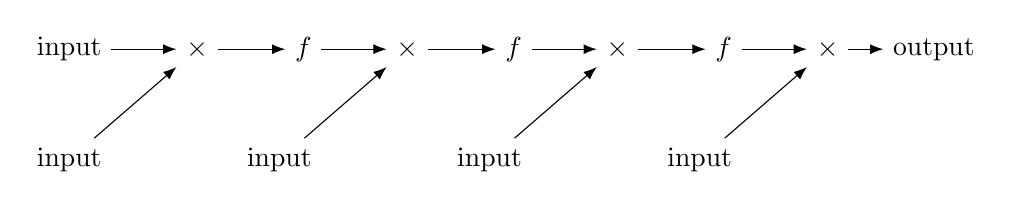
\begin{tikzpicture}[level distance=3.1em, sibling distance=4em,edge from parent/.style={draw,Latex-},left]
		\node{output}[grow=left]
		child{node{$\times$}%[level distance=4em]
			child[missing]{}
			child{node{$f$}
				child{node{$\times$}
					child[missing]{}
%					child{node{\begin{tabular}{c}do\\something\end{tabular}}
					child{node{$f$}
						child{node{$\times$}
							child[missing]{}
							child{node{$f$}
								child{node{$\times$}%[level distance=3em]
									child[missing]{}
									child{node{input}}
									child{node{input}}
								}
							}
							child{node{input}}
						}
					}
					child{node{input}}
				}     	
			}
			child{node{input}
			}
		};
		\end{tikzpicture}
	\end{center}
	\caption[Flowchart of a calculation dependency]{A calculation dependency, where $f$ is some function and $\times$ is something like multiplication.}\label{fig:depends}
\end{figure}


\subsection{sig}
There is nothing so new here, but it helps to write this function's calculation out to fix notation for when we come to the derivative.

\verb|sig(A,m)| calculates the signature of a piecewise linear path by combining the signatures of each straight-line-piece (which are the exponents of the displacement) using Chen's formula. 

If the $d$-dimensional input was $\big((p_{jk})_{j=0}^l\big)_{k=1}^d$ %there must be some better way to write this input.
 I could express the calculation like this. The displacement vectors are given by
\begin{align}
(q_j)_k &= p_{jk}-p_{(j-1),k} \\%&\text{(displacement)}\\
\shortintertext{and the signature of the $j$ segment is}
r_j(i_1\dots i_n) &= \frac1{n!}\prod_{h=1}^n(q_j)_{i_h}\label{eq:exp}\\%&\begin{matrix}\text{segment signature calculated}\\\text{for all words up to length $m$}\end{matrix}
\shortintertext{and using Chen's relation we find the signature of the path up to point $j$}
s_1(i_1\dots i_n) &= r_1(i_1\dots i_n) \nonumber
\\
s_j(i_1\dots i_n) &= s_{j-1}(i_1\dots i_n)+\left[\sum_{p=1}^{n-1} s_{j-1}(i_1\dots i_p)r_j(i_{p+1}\dots i_n)\right]+r_j(i_1\dots i_n).\\%&\begin{matrix}\text{signature of the path}\\\text{up to point $j$}\end{matrix}
%\shortintertext{If you'll tolerate an invalid ellipsis as an empty word and remember that the signature of an empty word is always 1, this can be written simply}
\shortintertext{I adopt the convention that a nonsensical ellipsis like $i_1\dots i_0$ means the empty word $\emptyword$. The value of a signature on the empty word is the scalar 1. This can therefore be written simply}
s_j(i_1\dots i_n)&= \sum_{p=0}^n s_{j-1}(i_1\dots i_p)r_j(i_{p+1}\dots i_n).\nonumber
\end{align}
Each signature object is calculated all at once (i.e.~its value for all words is calculated in one go, for all words up to length $m$), and stored in a vector (one for each level/length of word) of vectors (of words in alphabetical order). The output of the function is all the values of $s_l$.
For example, for a path given as six points, the calculation dependency looks like \autoref{fig:sigdepend}, taking the displacement vectors and signature objects as single entities and neglecting the actual calculation of the displacements. The calculation order needn't be like this, the tree could be constructed differently, but the number of operations would be unchanged. A nested calculation order like this requires only storing one $s_j$ at a time.
\begin{figure}[h]
\begin{center}
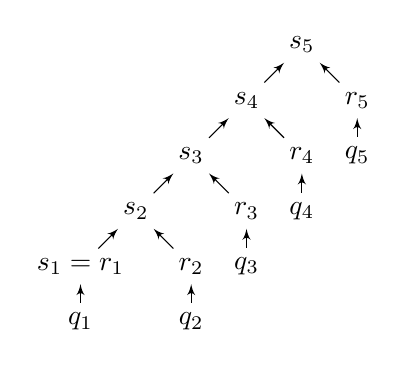
\begin{tikzpicture}[level distance=2em, sibling distance=4em,edge from parent/.style={draw,latex'-}]
\node{$s_5$}
  child{node{$s_4$}
    child{node{$s_3$}
      child{node{$s_2$}
        child{node{$s_1=r_1$}
          child{node{$q_{1}$}
%            child{node{$p_{0\cdot}$}}
%            child{node{$p_{1\cdot}$}}
          }
        }
      child{node{$r_2$}
        child{node{$q_2$}
%          child{node{$p_{1\cdot}$}}
%		  child{node{$p_{2\cdot}$}}
        }
      }
    }
    child{node{$r_3$}
      child{node{$q_3$}
%        child{node{$p_{2\cdot}$}}
%        child{node{$p_{3\cdot}$}}
      }
    }
  }     	
  child{node{$r_4$}
    child{node{$q_4$}}  	
  }
}
child{node{$r_5$}
  child{node{$q_5$}}
};
\end{tikzpicture}
\end{center}
\caption{Sig calculation dependency}\label{fig:sigdepend}
\end{figure}
%	\Tree [.{chen} [.{chen} [.{chen} [.{chen} [.{exp} $\vec x_1$ ] [.{$\exp$} $\vec x_2$ ] ] [.{exp} {$\vec x_3$} ] ] [.{exp} {$\vec x_4$} ] ] [.{exp} {$\vec x_5$} ] ]

I use the $\kron$\index{tensor@$\kron$} symbol for the Kronecker product of two column vectors as a vector, which takes a vector of length $x$ and a vector of length $y$ to a vector of length $xy$.
If $u$ has length $x$ and $v$ has length $y$ then $uv$ has elements $(u\kron v)_{(i-1)y+j}=u_iv_j$.
If $a$ is a signature, then I write $a^m$\jindmath{a^m}{am} for the vector of its elements at level $m$.
To calculate $r_j$ I use the procedure in \autoref{alg:segsignature} and the algorithm for the full signature is \autoref{alg:sig}.
\begin{algorithm}\caption{Segment signature\label{alg:segsignature}}
\begin{algorithmic}[1]
	\State $r_j^1\gets q_j$
	\For {$n\gets 2,m$}
	\State $r_j^n\gets \frac1{n}(r_j^{n-1}\kron q_j)$
	\EndFor
\end{algorithmic}
\end{algorithm}
\begin{algorithm}\caption{sig\label{alg:sig}}
\begin{algorithmic}[1]
	\State Calculate $r_1$
	\For {$n\gets 1,m$}%{$n\in\{1,\dots,m\}$ }
	\State $s^n\gets r_1^n$
	\EndFor
	\For {$j\gets 2,l$}
	\State Calculate $r_j$
	\For {$n\gets m,1$}	\Comment make $s^n$ go from being $s^n_{j-1}$ to $s^n_j$
	\For {$n'\gets (n-1),1$}
	\State $s^{n}\gets s^{n}+s^{n'}\kron r_j^{n-n'}$
	\EndFor
	\State $s^{n}\gets s^{n}+r_j^n$
	\EndFor
	\EndFor
	\State $s^{n}$ is now $s_l^n$ for each $n$
\end{algorithmic}
\end{algorithm}

\def\pbinomjr#1#2{\left(\begin{smallmatrix}#1\\#2\end{smallmatrix}\right)}
It feels wasteful to store each $r_j^n$ as a whole vector of $d^n$ numbers, because they are really repeats. The signature of a straight line takes the same value on all permutations of a word, so there are only $\pbinomjr{d+n-1}{n}$ distinct values. %"multichoose"
But trying to exploit this led me to slower, more complicated code.

\subsection{sigbackprop}
Naively, given a calculation tree to define an output in terms of simple calculations, we can backpropagate derivatives through the tree using the chain rule. If we know the value of every node in the tree (having stored them while calculating the output) then we can pass a derivative though each leg of a multiplication node $M$ by multiplying it by the stored values in the other inputs to $M$. We send a derivative both ways through an addition unchanged. 
There is naturally a time/memory tradeoff in such a calculation, because each value could just be recalculated from inputs when it is needed, instead of having been remembered. We can in fact do much better than storing all the intermediate values, or even just all the $s_j$.

In general, if $X$ is the signature of a path $\gamma$, then the signature $X'$ of the reversed path $\gamma^{-1}$ is a permutation with some elements negated. It is the image of $X$ under $\alpha$, the antipode of the concatenation algebra (page~19 of \cite{FLA}).
\begin{align}
X'(a_1\dots a_n)=(-1)^nX(a_n \dots a_1)
\end{align}
%Considering each signature level as a vector, this is a permutation of elements.
If $\gamma$ is a straight line, then the component of the signature is the same on all permutations of a word, and so we have the simpler
\begin{align}
X'(a_1\dots a_n)=(-1)^nX(a_1\dots a_n) \label{eq:loseStraightSeg}
\end{align}
%\def\rr#1{\tilde r_{#1}}
Because all the $r_j$ are easy to calculate as the difference of inputs, we can easily use this to calculate $s_{j-1}$ from $s_j$. This we can perform at the same time as the backpropagation of derivatives with respect to $s_j$.
Let the vector containing level $n$ of $r_j$ be $r_j^n$, with the derivatives with respect to its elements being $R_j^n$. Similarly $s_j^n$ and $S_j^n$ for $s_j$. 

It is convenient to define the corresponding backpropagation operations to $\kron$. If $u$ has length $x$, $v$ has length $y$, and $w$ has length $xy$, then $w\underleftarrow\otimes v$\index{tensora@$\underleftarrow\otimes$}
has length $x$ with elements $(w\underleftarrow\otimes v)_i=\sum_jw_{(i-1)y+j}v_j$ and $u\underrightarrow\otimes w$ \index{tensor b@$\underrightarrow\otimes$}
has length $y$ with elements $(u\underrightarrow\otimes w)_j=\sum_i u_iw_{(i-1)y+j}$.
%\newpage
Then the algorithm, based in the function \verb|sigBackwards|, proceeds as shown in \autoref{alg:sigbackwards}. Some of the same logic is used for \verb|sigjoinbackprop|.
\iffalse
\begin{algorithm}\caption{sigBackwards\label{alg:sigbackwards}}
\begin{algorithmic}[1]
	%\State $s\gets s_l$, calculated using \verb|sig|
	\For {$n\gets 1,m$}%{$n\in\{1,\dots,m\}$ }
	\State $s^n\gets s_l^n$, calculated using \verb|sig|
	\State $S^n\gets S_l^n$, an input
	\EndFor
	\For {$j\gets l,1$}
	\Statex $\quad$ ($s^n$ is now $s^n_{j}$ and $S^n$ is now $S^n_j$ for each $n$.)
	\State Calculate $r_j$.
	\For {$n\gets m,1$}	%\Comment make $s^n$ go from being $s^n_j$ to $s^n_{j-1}$
	\For {$n'\gets (n-1),1$}
	\State $s^{n}\gets s^{n}+(-1)^{n-n'}s^{n'}\kron r_j^{n-n'}$
	\EndFor
	\State $s^{n}\gets s^{n}+(-1)^{n}r_j^n$
	\EndFor
	\Statex $\quad$ ($s^n$ is now $s^n_{j-1}$ for each $n$.)
	\Statex $\quad$ Calculate $R_j$ as follows:
	\For {$n\gets 1,m$}	%\Comment Calculate $R_j$
	\State $R^n\gets S^n$
	\EndFor
	\For {$n\gets 1,m$}	%\Comment Calculate $R_j$
	\For {$n'\gets (n-1),1$}
	\State $R^{n-n'}\gets R^{n-n'} + s^{n'}\underrightarrow\otimes S^{n}$
	\EndFor
	\EndFor
	\Statex $\quad$ ($R^n$ is now $R^n_{j}$ for each $n$.)
	\State Backpropagate $R^n_j$ through (\ref*{eq:exp}).
	\Statex $\quad$ Calculate $S_{j-1}$ as follows:
	\Statex \Comment \begin{minipage}{0.5\textwidth}(We could calculate $S_{j-1}$ just like we calculated $R_j$,\\
	but we can just update the $S^n$ in place.)\end{minipage}% to make them go from being $S^n_j$ to $S^n_{j-1}$.)
	\For {$n'\gets 1,(m-1)$}	
    \For {$n\gets (n'+1,m)$}
    \State $S^{n'}\gets S^{n'} + S^{n}\underleftarrow\otimes r^{n-n'}$
    \EndFor
    \EndFor
    \Statex $\quad$ ($S^n$ is now $S^n_{j-1}$ for each $n$.)
	\EndFor

\end{algorithmic}
\end{algorithm}
\fi 
%Nested algorithms seem to fail - I think there is only one set of variables in the package. Saveboxes save the day.
\newsavebox{\inneralga}
\newsavebox{\inneralgb}
\newsavebox{\inneralgc}
\savebox{\inneralga}{$\left\{\begin{minipage}{0.5\textwidth}\begin{algorithmic}
	\For {$n\gets m,1$}	%\Comment make $s^n$ go from being $s^n_j$ to $s^n_{j-1}$
	\For {$n'\gets (n-1),1$}
	\State $s^{n}\gets s^{n}+(-1)^{n-n'}s^{n'}\kron r_j^{n-n'}$
	\EndFor
	\State $s^{n}\gets s^{n}+(-1)^{n}r_j^n$
	\EndFor
	\end{algorithmic}\end{minipage}\right.$}
\savebox{\inneralgb}{$\left\{\begin{minipage}{0.5\textwidth}\begin{algorithmic}
	\For {$n\gets 1,m$}	%\Comment Calculate $R_j$
	\State $R_j^n\gets S^n$
	\EndFor
	\For {$n\gets 1,m$}	%\Comment Calculate $R_j$
		\For {$n'\gets (n-1),1$}
			\State $R_j^{n-n'}\gets R_j^{n-n'} + s^{n'}\underrightarrow\otimes S^{n}$
		\EndFor
	\EndFor
\end{algorithmic}\end{minipage}\right.$}
\savebox{\inneralgc}{$\left\{\begin{minipage}{0.5\textwidth}\begin{algorithmic}
	\For {$n'\gets 1,(m-1)$}	
	\For {$n\gets (n'+1,m)$}
	\State $S^{n'}\gets S^{n'} + S^{n}\underleftarrow\otimes r^{n-n'}$
	\EndFor
	\EndFor
	\end{algorithmic}\end{minipage}\right.$}

\begin{algorithm}\caption{sigBackwards\label{alg:sigbackwards}}
	\begin{algorithmic}[1]
		%\State $s\gets s_l$, calculated using \verb|sig|
		\For {$n\gets 1,m$}%{$n\in\{1,\dots,m\}$ }
		\State $s^n\gets s_l^n$, calculated using \verb|sig|
		\State $S^n\gets S_l^n$, an input
		\EndFor
		\For {$j\gets l,1$}
		\Statex $\quad$ ($s^n$ is now $s^n_{j}$ and $S^n$ is now $S^n_j$ for each $n$.)
		\State Calculate $r_j$.
		\State \parbox{1.4in}{Use \hbox{(\ref*{eq:loseStraightSeg})} to make $s^n$ be $s^n_{j-1}$ for each $n$.}\hfill{\usebox{\inneralga}}
		\Statex
		\Statex
		\State Calculate $R_j$.\hfill{\usebox{\inneralgb}}
		\State Backpropagate $R^n_j$ through (\ref*{eq:exp}).
		\State \parbox{1.4in}{\raggedright Make $S^n$ be $S^n_{j-1}$, doable in place.}\hfill\usebox{\inneralgc}
		%\Statex \Comment \begin{minipage}{0.5\textwidth}(We could calculate $S_{j-1}$ just like we calculated $R_j$,\\
		%	but we can just update the $S^n$ in place.)\end{minipage}% to make them go from being $S^n_j$ to $S^n_{j-1}$.)

		%\Statex $\quad$ ($S^n$ is now $S^n_{j-1}$ for each $n$.)
		\EndFor
		
	\end{algorithmic}
\end{algorithm}
%\newpage
%\afterpage{\clearpage}
%\clearpage
\subsection{sigscalebackprop}
%For this section to be all on one page is a good idea
Here we present a general sensible idea to use when differentiating products of terms sampled with replacement from a list: \emph{you keep the simple code you would have written if replacement was not allowed}.

Consider \verb|sigscalebackprop| called in $d$ dimensions up to level $m$, in particular its action for a single level $l\le m$. Each level's calculation produces derivatives with respect to its part of the original signature, and contributes to derivatives with respect to the scales.
The data are $a$, the $l$th level of the original signature, $b$, the scales, %$B$ the to-be-incremented derivatives with respect to $b$,
 and $E$, the supplied derivatives with respect to the $l$th level of the output.  Denote the output of the expression by $e$ and the to-be-calculated derivatives with respect to $a$ and $b$ by $A$ and $B$ respectively. I denote subscripting of the inputs and outputs with square brackets, and unlike earlier where I indexed a level of a signature as a vector, here I am indexing it as a tensor.
 
The expression to be differentiated is as follows.
\begin{align}
	e[i_1,\dots,i_l]&=\Big(\prod_{j=1}^l b[i_j]\Big)a[i_1,\dots,i_l]&\text{for}\quad (i_1,\dots,i_l)\in\{1,\dots,d\}^l\label{eq:orig}
%\end{align}
\shortintertext{Using standard rules for differentiation, the derivative calculations are as follows.}
%\begin{align}
A[i_1,\dots,i_l]&=\Big(\prod_{j=1}^l b[i_j]\Big)E[i_1,\dots,i_l]&\text{for}\quad (i_1,\dots,i_l)\in\{1,\dots,d\}^l\\
B[k]&=\sum_{\substack{(i_1,\dots,i_l)\in\\\{1,\dots,d\}^l}}B[k;i_1,\dots ,i_l]&\text{for}\quad k\in\{1,\dots,d\},\\\shortintertext{where the single contribution of a product is}%\nonumber\\
B[k;i_1,\dots,i_l]&=\Big(\prod_{\substack{j=1\\i_j\ne k}}^l b[i_j]\Big)a[i_1,\dots,i_l]\mathrlap{E[i_1,\dots,i_l]\;C^k_{i_1\dots i_l}b[k]^{C^k_{i_1\dots i_l}-1}}%\text{for}\quad k\in\{1,\dots,d\}
%\end{align}
\shortintertext{and $C^k_{i_1\dots i_l}$ is the number of $j$ for which $i_j=k$.
%THESE NEWLINES LOOK FINE BUT GENERATE UNDERFULL HBOX WARNINGS
\newline\newline %http://tex.stackexchange.com/questions/280681/how-to-have-multiple-lines-of-intertext-within-align-environment
Evaluating $e$ according to (\ref*{eq:orig}) will take time $d^{l}l$ but evaluating $B$ naively according to this procedure takes at least $d^{l+1}d$, because evaluating the $d$ counts $C^\cdot_{i_1\dots i_l}$ requires $d$ time for every $(i_1\dots i_l)$, even though most are zero. A couple of rearrangements:}
%\begin{align}
B[k;i_1,\dots,i_l]&=\Big(\prod_{j=1}^l b[i_j]\Big)a[i_1,\dots,i_l]\mathrlap{E[i_1,\dots,i_l]\;C^k_{i_1\dots i_l}b[k]^{-1}}%\text{for}\quad k\in\{1,\dots,d\}
\\B[k;i_1,\dots,i_l]&=\mathrlap{\sum_{h=1}^l1_{\{i_{h}=k\}}\Big(\prod_{j=1}^l b[i_j]\Big)a[i_1,\dots,i_l]E[i_1,\dots,i_l]\;b[i_h]^{-1}}
\end{align}
Organising the terms differently by making $k$ range among $(i_1,\dots,i_l)$ instead of $\{1,\dots,d\}$ means we split the $C_\cdot^\cdot$ occurrences of each multiplication. This leads to \autoref{alg:sigscalebp}, which only takes time $d^ll$.
\begin{algorithm}\caption{\label{alg:sigscalebp}single level of sigscalebackprop}
\begin{algorithmic}[1]
	\For {$(i_1,\dots,i_l)\in\{1,\dots,d\}^l$ }
	\State $\displaystyle prod\gets\prod_{j=1}^lb[i_j]$
	\State $A[i_1,\dots,i_l]\gets prod\;E[i_1,\dots,i_l]$
	\For {$h\in\{1,\dots,l\}$ }
	\State $B[i_h]\gets B[i_h]+prod\;a[i_1,\dots,i_l]E[i_1,\dots,i_l]/b[i_h]$
	\EndFor
	\EndFor
\end{algorithmic}
\end{algorithm}

\endDocumentJR
